% Appendix C

\chapter{Orquestación de los flujos meteorológicos} % Main appendix title

\label{AppendixC}

En este apéndice se presentan los pipelines de Fabric que orquestan la transferencia de los datos meteorológicos observados y de los pronósticos meteorológicos desde la capa~1 hacia la capa~2, descritos en las secciones~\ref{subsec:pipeline_meteorologico} y \ref{subsec:pipeline_pronosticos}.

%----------------------------------------------------------------------------------------
\section{Datos meteorológicos observados}
\label{sec:apendice_ppln_meteo}
%----------------------------------------------------------------------------------------

La figura \ref{fig:pipeline_meteo} presenta el pipeline \code{PPLN\_METEO}.

\begin{figure}[H]
	\centering
	\resizebox{\textwidth}{!}{%
		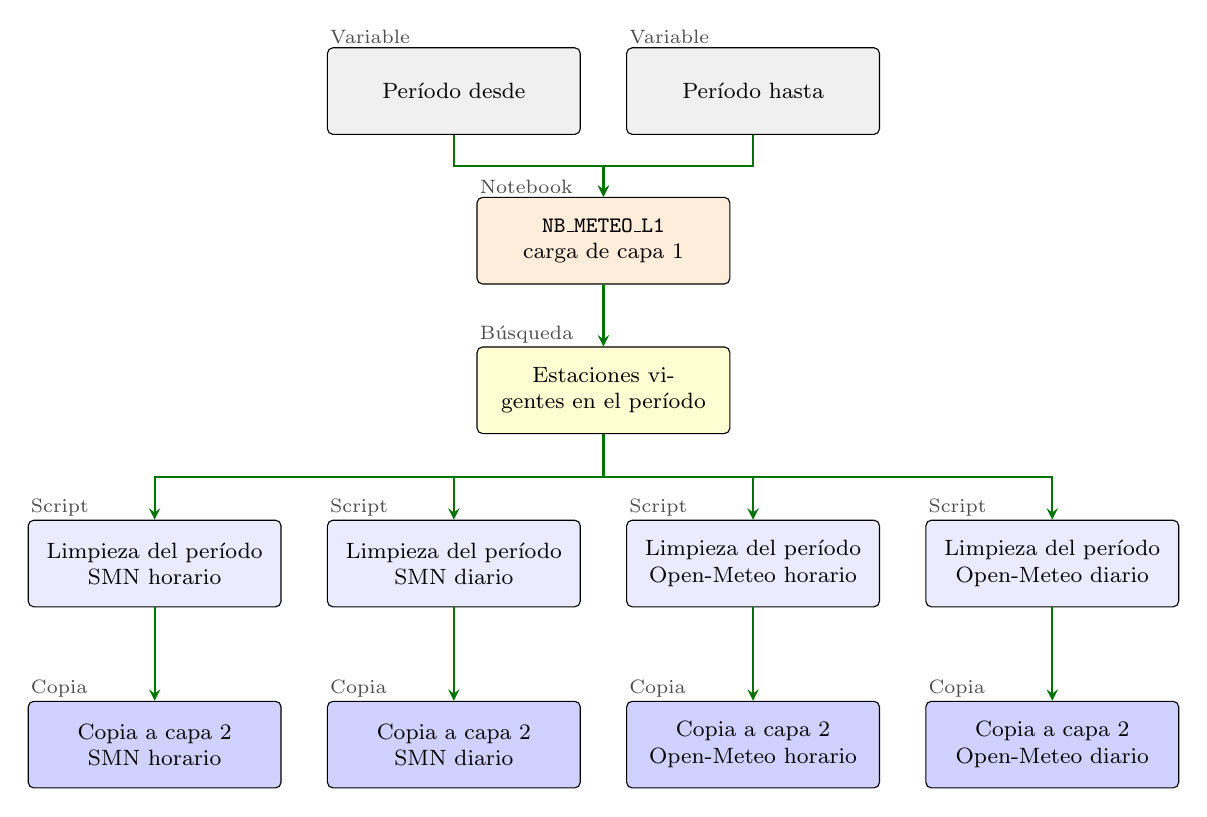
\begin{tikzpicture}[
			font=\footnotesize,
			act/.style={draw, rounded corners=2pt, align=center, fill=white, text width=3.0cm,
				minimum height=1.1cm, inner sep=3pt},
			var/.style={act, fill=gray!12},
			nb/.style={act, fill=orange!14},
			busq/.style={act, fill=yellow!18},
			script/.style={act, fill=blue!8},
			copia/.style={act, fill=blue!18},
			falla/.style={act, fill=red!12},
			tipo/.style={font=\scriptsize, text=gray!60!black, anchor=south west, inner sep=1pt},
			ok/.style={-stealth, thick, green!45!black},
			linea/.style={thick, green!45!black},
			comp/.style={-stealth, thick, dashed, blue!60!black},
			err/.style={-stealth, thick, red!70!black}
			]
			% Variables y notebook de capa 1
			\node[var] (v1) at (3.8,0) {Período desde};
			\node[var] (v2) at (7.6,0) {Período hasta};
			\node[nb] (nb) at (5.7,-1.9) {\texttt{NB\_METEO\_L1}\\carga de capa 1};
			\node[busq] (est) at (5.7,-3.8) {Estaciones vigentes en el período};
			% Ramas por tabla de capa 2
			\foreach \x/\n/\t in {0/s1/SMN horario, 3.8/s2/SMN diario, 7.6/s3/Open-Meteo horario, 11.4/s4/Open-Meteo diario} {
				\node[script] (\n) at (\x,-6.0) {Limpieza del período\\\t};
				\node[copia] (c\n) at (\x,-8.3) {Copia a capa 2\\\t};
				\draw[ok] (\n) -- (c\n);
				\draw[ok] (est.south) -- (5.7,-4.9) -| (\n.north);
			}
			% Etiquetas de tipo de actividad
			\foreach \n/\t in {v1/Variable, v2/Variable, nb/Notebook, est/Búsqueda, s1/Script, s2/Script, s3/Script, s4/Script, cs1/Copia, cs2/Copia, cs3/Copia, cs4/Copia}
				\node[tipo] at (\n.north west) {\t};
			% Dependencias
			\draw[ok] (v1.south) -- (3.8,-0.95) -| (nb.north);
			\draw[ok] (v2.south) -- (7.6,-0.95) -| (nb.north);
			\draw[ok] (nb) -- (est);
		\end{tikzpicture}%
	}
	\caption{Pipeline de Fabric para la orquestación de datos meteorológicos observados.}
	\label{fig:pipeline_meteo}
\end{figure}

Para los datos horarios del SMN, la actividad de copia filtra el rango de fechas, conserva las estaciones vigentes y construye la marca temporal \code{FECHA\_HORA}. También ajusta la numeración horaria para compatibilizarla con la convención utilizada en CAMMESA. A partir de la temperatura, la humedad relativa y la velocidad del viento observadas, junto con la radiación de Open-Meteo, se calcula la temperatura aparente según la ecuación~\ref{eq:temp_aparente}. Finalmente, las variables se redondean y tipifican antes de escribirlas en el esquema \code{METEO} del warehouse.

%----------------------------------------------------------------------------------------
\section{Pronósticos meteorológicos}
\label{sec:apendice_ppln_pronos}
%----------------------------------------------------------------------------------------

La figura \ref{fig:pipeline_pronos} presenta el pipeline \code{PPLN\_PRONOS}. Los notebooks de Open-Meteo y TWC y la validación del SMN se ejecutan en paralelo. Luego, cada tabla de capa~2 se actualiza mediante la eliminación previa del período a insertar y una actividad de copia desde la base KQL.

\begin{figure}[H]
	\centering
	\resizebox{12.5cm}{!}{%
		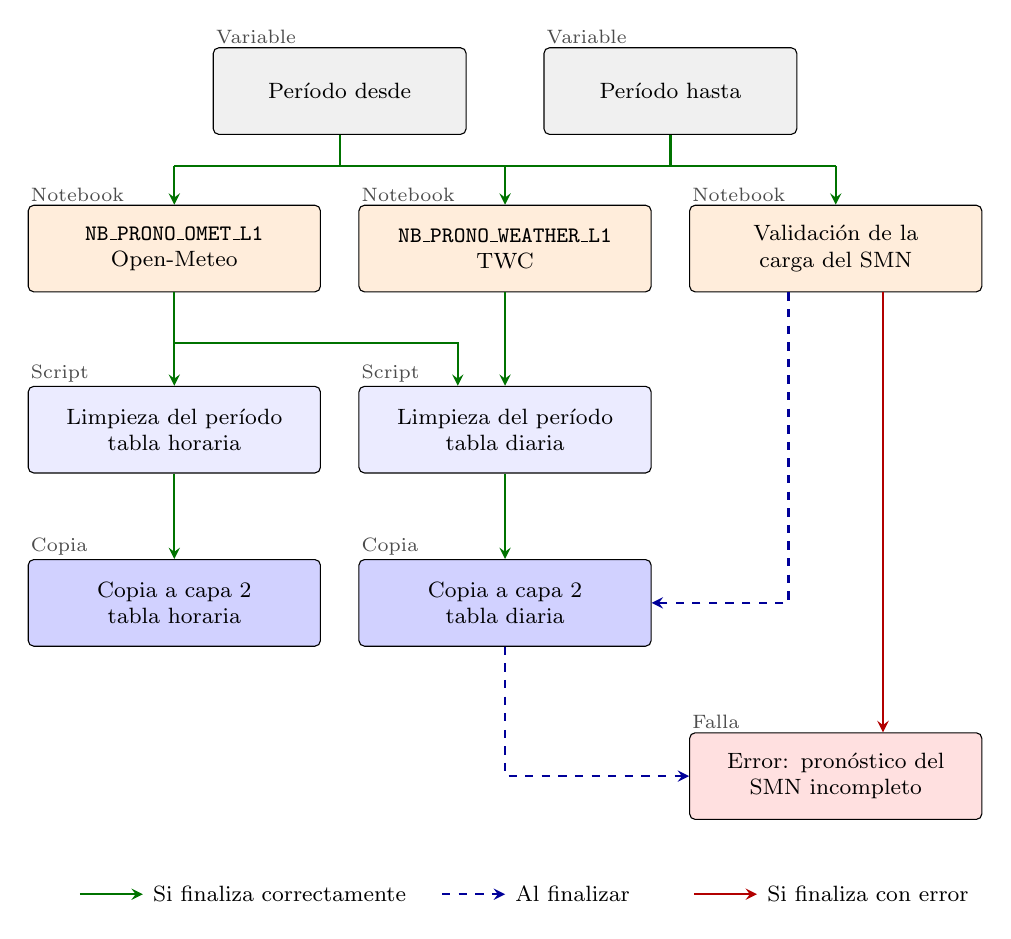
\begin{tikzpicture}[
			font=\footnotesize,
			act/.style={draw, rounded corners=2pt, align=center, fill=white, text width=3.0cm,
				minimum height=1.1cm, inner sep=3pt},
			var/.style={act, fill=gray!12},
			nb/.style={act, fill=orange!14},
			busq/.style={act, fill=yellow!18},
			script/.style={act, fill=blue!8},
			copia/.style={act, fill=blue!18},
			falla/.style={act, fill=red!12},
			tipo/.style={font=\scriptsize, text=gray!60!black, anchor=south west, inner sep=1pt},
			ok/.style={-stealth, thick, green!45!black},
			linea/.style={thick, green!45!black},
			comp/.style={-stealth, thick, dashed, blue!60!black},
			err/.style={-stealth, thick, red!70!black}
			]
			% Variables
			\node[var] (v1) at (2.1,0) {Período desde};
			\node[var] (v2) at (6.3,0) {Período hasta};
			% Capa 1 y validación
			\node[nb, text width=3.5cm] (om) at (0,-2.0) {\texttt{NB\_PRONO\_OMET\_L1}\\Open-Meteo};
			\node[nb, text width=3.5cm] (tw) at (4.2,-2.0) {\texttt{NB\_PRONO\_WEATHER\_L1}\\TWC};
			\node[nb, text width=3.5cm] (va) at (8.4,-2.0) {Validación de la carga del SMN};
			% Capa 2
			\node[script, text width=3.5cm] (lh) at (0,-4.3) {Limpieza del período\\tabla horaria};
			\node[script, text width=3.5cm] (ld) at (4.2,-4.3) {Limpieza del período\\tabla diaria};
			\node[copia, text width=3.5cm] (ch) at (0,-6.5) {Copia a capa 2\\tabla horaria};
			\node[copia, text width=3.5cm] (cd) at (4.2,-6.5) {Copia a capa 2\\tabla diaria};
			\node[falla, text width=3.5cm] (fa) at (8.4,-8.7) {Error: pronóstico del SMN incompleto};
			% Etiquetas de tipo de actividad
			\foreach \n/\t in {v1/Variable, v2/Variable, om/Notebook, tw/Notebook, va/Notebook, lh/Script, ld/Script, ch/Copia, cd/Copia, fa/Falla}
				\node[tipo] at (\n.north west) {\t};
			% Dependencias desde las variables
			\draw[linea] (v1.south) -- (2.1,-0.95);
			\draw[linea] (v2.south) -- (6.3,-0.95);
			\draw[linea] (0,-0.95) -- (8.4,-0.95);
			\foreach \n/\x in {om/0, tw/4.2, va/8.4}
				\draw[ok] (\x,-0.95) -- (\n.north);
			% Tabla horaria
			\draw[ok] (om) -- (lh);
			\draw[ok] (lh) -- (ch);
			% Tabla diaria
			\draw[ok] (om.south) -- (0,-3.2) -| ([xshift=-6mm]ld.north);
			\draw[ok] (tw) -- (ld);
			\draw[ok] (ld) -- (cd);
			\draw[comp] ([xshift=-6mm]va.south) |- (cd.east);
			% Falla
			\draw[err] ([xshift=6mm]va.south) -- ([xshift=6mm]fa.north);
			\draw[comp] (cd.south) |- (fa.west);
			% Leyenda
			\draw[ok] (-1.2,-10.2) -- (-0.4,-10.2) node[right, text=black] {Si finaliza correctamente};
			\draw[comp] (3.4,-10.2) -- (4.2,-10.2) node[right, text=black] {Al finalizar};
			\draw[err] (6.6,-10.2) -- (7.4,-10.2) node[right, text=black] {Si finaliza con error};
		\end{tikzpicture}%
	}
	\caption{Pipeline de Fabric para la orquestación de pronósticos meteorológicos.}
	\label{fig:pipeline_pronos}
\end{figure}
